Loi de Faraday. Un champ électrique (courant) est induit le long de boucles qui entourent la surface traversée par un champ magnétique variable dans le temps.

Forme différentielle:

\[
\nabla \times \boldsymbol{E} = - \frac{\partial{\boldsymbol{B}}}{\partial{t}}\]

Forme intégrale:

\[
\oint \boldsymbol{E} \cdot \mathrm{d}\boldsymbol{l} = -\frac{\mathrm{d}}{\mathrm{d}t} \iint_S \boldsymbol{B}\cdot \mathrm{d}\boldsymbol{S}
\]

\tikzstyle{fleche}=[->,line width=1pt]
\begin{tikzpicture}
  \begin{scope}[xshift=0 cm,yshift=0 cm, scale = 1.6]%
\foreach \t in {60,120, ...,360}
\draw [fleche] (\t:1) -- (\t:2.8);
\foreach \t in {30,90, ...,360}
\draw [fleche] (\t:2) -- (\t:2.45);
\foreach \t in {15,45, ...,360}
\draw [fleche] (\t:3) -- (\t:3.2);
\draw (0,0) circle(0.1) node [above right] {$Q$};
  \end{scope}
\end{tikzpicture}
\vfill
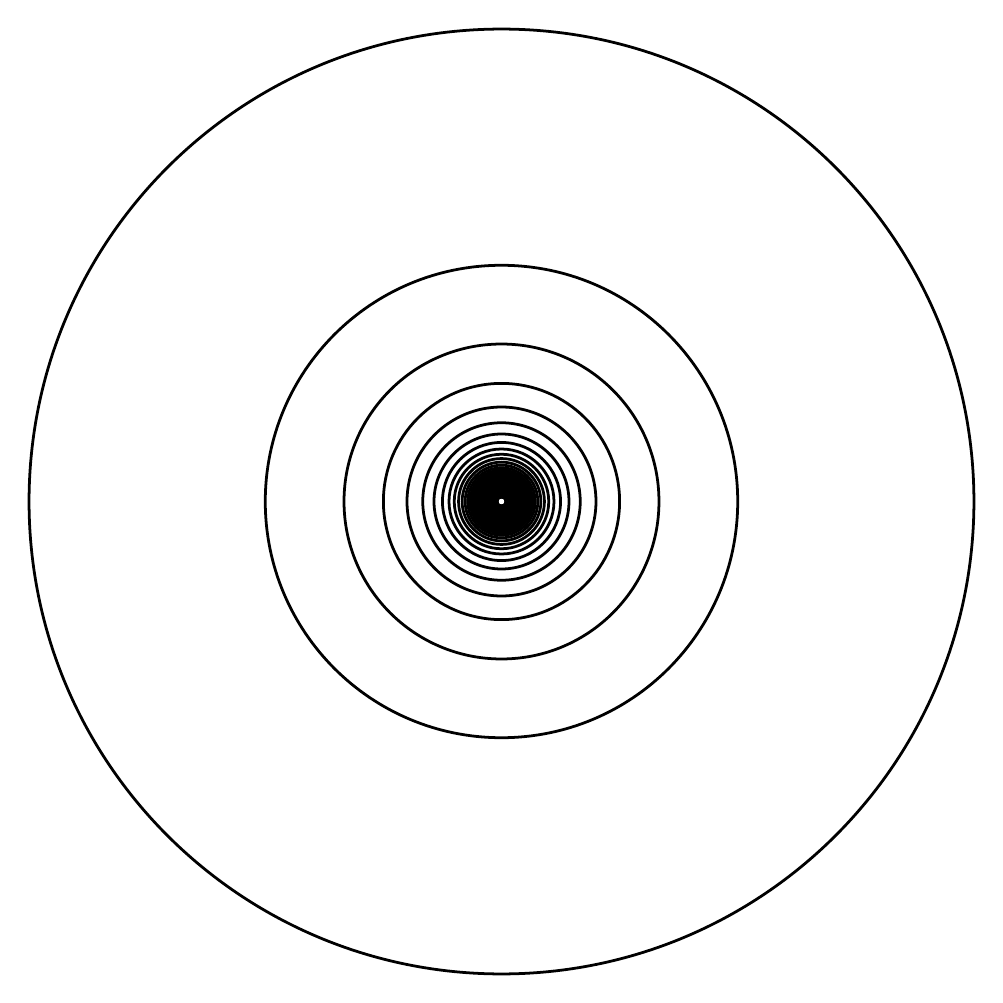
\begin{tikzpicture}
  \begin{scope}[xshift=0 cm,yshift=0 cm, scale = 1]%
\foreach \t in {1,2, ...,100}
\draw [line width=1pt] (0,0) circle (6/\t) ;
  \end{scope}
\end{tikzpicture}




%%%%%%%%%%%%%%%%%%%%%%%%%%%%%%%%%%%%%%%%%%%%%%%%%%%%%%%%%%%%%%%%%%%%%%%%%%%%
